\chapter{Discussion}
\label{chap:discussion}

In this work, an approach towards modelling run-of-the-river power plants and simulating electricity generation based on open access geodatabases was put forward. In this chapter, we will examine to what extent the model and the simulation process fit the specifications defined in Sec. \ref{sub:spec}, discuss their potential applications, their limits, and give some ideas to improve the results.
\section{Consistency with the specifications}

The objectives of this work (see Sec. \ref{sub:spec}) were to be able to obtain feed-in time series both from single plants and for large areas and to be compatible with the environment data sets of the OEDB (runoff, river network, ...). The developed model (Ch. \ref{chap:simulation_model}), together with the guidelines on preprocessing the data (Sec. \ref{sec:data_preproc}), meet these requirements and allows the user to run simulations with various degrees of precision in the input data. However, it was difficult to assess the proper functioning of the model, due to the limited availability of production data. This is discussed further in Sec. \ref{sec:limits}.

\section{Applications of the model}

The model, after being completed following the guidelines given in Sec. \ref{sec:improv} and validated, could find applications at different levels. It could be a useful tool for an individual or a society seeking to build a run-of-the-river plant, as it reproduces the design process of a plant. The parameters related to human and economic decisions, such as the percentage of the year the plant should run at full load, can be changed to personalize the process. This is also true of legal parameters such a the residual water flow. \newline
It can also be useful to research institutes or public bodies looking for a way to run state-wide simulations with little information about the plants installed. It could as well be integrated in energy systems modelling and optimization tools.

\section{Limits of the model}
\label{sec:limits}
If the model fulfills the conditions set in the specifications, the chapter presenting the results (Ch. \ref{chap:results}) was not conclusive, and failed to lead to a validation of the model.
\subsection{Simulation from precise data}
\label{sub:lim_single}
The single plant simulation over-estimates the production from April to July. This is normal, as the first months of production were a running-in phase, during which the plant did not work to its full capacity. However, the simulated production for August is less than the measured production. This could be due to the very low water flows measured in August: the usable water flow is often under the minimal waterflow of the turbine, which in the model does not produce any power. In reality however the dam is used to retain water upstream from the turbine and release it when it is sufficient to set it in motion. Ideas on how to include this behaviour in the model are given in Sec. \ref{sub:impoudment}.

\subsection{Extrapolation of missing data}
\label{sub:lim_extra}
Section \ref{sec:missing_data} showed that values very far from the reality were assigned to the plants during the extrapolation process when done on the wrong runoff values (gauge station located on another river or far away from the plant, or raster cell not matching the river course). However, the assignment of an oversized nominal water flows leads to the assignment of a proportionally undersized water head. Thus, the power output stays consistent, as long as the runoff time series vary in the same order of magnitude as the river the plant should have been assigned to. Ideas on how to improve the assignment to raster cells and gauge stations are given in Sec. \ref{sub:imp_assign_cell} and Sec. \ref{sub:imp_assign_gauge}.

\subsection{Simulation based on limited data}
\label{sub:lim_data}
The state wide simulations run on Thuringia under-estimate the production. Since they sum the productions from individual plants and use the extrapolation process, they are naturally subject to the uncertainties mentioned in Sec. \ref{sub:lim_single} and Sec. \ref{sub:lim_extra}. In addition, the comparison with the production data from the AEE is biased since it is not based on the same technologies as the OPSD, and since the installed capacity from these two sources are different. The need for better input and validation data is developed in Sec. \ref{sub:imp_data}.

\subsection{Other uncertainties}
\label{sub:limits_others}

In order to simplify the model, assumptions were made in the choice or calculation of simulation parameters. These assumptions, listed below, can also cause errors in the simulation results. 
\begin{itemize}
 \item Calculation of \.V\textsubscript{res} according to \cite{pacer}. As explained in Sec. \ref{sub:extrapol_dV_res}, the residual water flow is fixed by law and therefore depends on the jurisdiction of the country or federal state. Some legal texts result in a constant value based on the type of river, while others define graded or dynamic residual water flows. According to Giesecke \cite{gies_qrest}, for the same plant and river characteristics, the residual water flow reduces the usable water flow by \unit{4}[\%] to \unit{50}[\%], depending on the legal text used to calculate it. Since the power output is proportional to the usable water flow, it is clear that the method used to calculate the residual water flow will have a big impact on the result. Solutions to improve the calculation of \.V\textsubscript{res} are discussed in Sec. \ref{sub:imp_dVres}.
 \item Calculation of \.V\textsubscript{n}. Section \ref{sub:extrapol_dV_n} showed how to extract the nominal water flow from the flow duration curve. The literature distinguishes isolated sites, for which the nominal water flow should be reached 250 days a year, and sites connected to the grid where the nominal water flow should be reached 50 to 90 days a year. In this work, the nominal water flows were chosen to be reached \unit[20]{\%} of the year (around 70 days) and even though this value seems coherent given the results from Sec. \ref{sec:missing_data}, it has a big influence on the overall production of a plant. The production of Thuringia from modelled runoffs was simulated over the year 2008, with different values for this percentage exceedence percentage:  with \unit[20]{\%} the yearly production is \unit[187]{GWh}, with \unit[30]{\%} it rises to \unit[210]{GWh} and with \unit[40]{\%} to \unit[223]{GWh}. Given the impact of this parameter, Sec. \ref{sub:imp_dVn} gives ideas on how to adjust its value to fit reality more precisely.
 \item Turbine type assignment. The type of turbine is extracted from the characteristic diagrams, depending on the nominal head and water flow of the turbine. However, Fig. \ref{charac_diag} shows that the characteristic diagrams of different turbine types partly overlap, and the overlapping zones are assigned arbitrarily to the first type tested (Sec. \ref{sub:get_type}). The error induced by this simplification is minor, because of the small difference between efficiency curves of the different types. However, ways of improving this process are presented in Sec. \ref{sub:imp_dVn}.
 \item Approximation of h with h\textsubscript{n}. Section \ref{sub:approx_h} justifies the approximation of h with h\textsubscript{n} due to the difficulty of calculating the water level directly downstream from the plant.  Like all approximations, this reduces the precision of the model. However, assessing the water level from the water flow would require to model precisely the bed of the river downstream from the plant. This task would be very time-consuming and would potentially require more approximations, it is therefore not certain that it would improve the result at all.
\end{itemize}


\section{Ways of improvement}
\label{sec:improv}

This work laid the foundations towards simulating run-of-the-river hydroelectricity within the openFRED project. Section \ref{sec:limits} and Ch. \ref{chap:results} identified the limits of the developed model in its current state. However, these problems can be addressed.

\subsection{Assignment to gauge stations}
\label{sub:imp_assign_gauge}
Section \ref{sub:lim_extra} mentioned the problems appearing in the extrapolation process when a plant is assigned to runoff time series not consistent with the river it is actually on. As explained there, this problem does not impact the simulated production much, as long as the runoff time series vary in the same order of magnitude as the river the plant should have been assigned to. In the case of measured runoffs, the situation arises when plants are located on rivers with no gauge station. With the assignment process described in Sec. \ref{sub:pp_reg}, when no gauge station is found on the same river as the plant, the closest gauge station is assigned. \newline
Instead of looking for the closest gauge, the assignment process could search for the next gauge downstream from the plant, based on the ``Gewässerkennzahl'' (GWK). The GWK is the identification number of each river in Germany, and is constructed hierarchically, so that each river can be traced back to its position in the river network. Each river basin has a specific number (1-Danube, 2-Rhine, 3-Ems, 4-Weser, 5-Elbe, 6-Oder, 9-Coastal region) and each tributary is assigned a GWK as follows:
\begin{itemize}
 \item The four main tributaries are assigned the numbers of their river basins (respectively river sections) followed by an even number from 2 to 8, 2 being the most upstream main tributary and 8 the most downstream.
 \item The river sections in between receive as final numbers uneven numbers from 1 (upstream section) to 9 (downstream section).
 \item The four main tributaries of each section are identified and the process starts over until each tributary has a number.
\end{itemize}
The process is illustrated in Fig. \ref{explain_gwk} and leads to a numbering system where all rivers have a GWK ending with an even number. With this numbering system, if a river does not have a gauge station, we can identify the river it contributes to by looking for the penultimate even number and search for a gauge station on this river. The water flow measured there is more likely to vary in the right order of magnitude than the water flow from a closer gauge station located on another river network.

\begin{figure}[H]
\centering
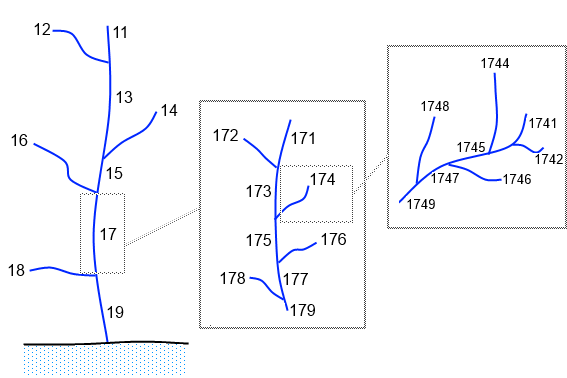
\includegraphics[width=9cm]{explain_gwk.png}
\caption{Illustration of the river numbering process in Germany}
\label{explain_gwk}
\end{figure}

\subsection{Assignment to raster cells}
\label{sub:imp_assign_cell}
The assignment problem is not limited to measured runoff. Section \ref{sec:missing_data} showed that some cells contain very low runoff data, even though they are located on the course of a river (see Fig. \ref{map_mosel_watergap}). This causes errors in the calculation of the nominal water flow and subsequently in the calculation of the nominal head, and the setting of the turbine type. Even though this does not have such a spectacular impact on the results as the differences in nominal water flows observed in Tab. \ref{tab_res_extra}, because they are compensated by a proportionally oversized head of water, more accurate results would be obtained by assigning coherent runoff values to each plant. \newline
A solution to achieve this would be to rebuild the network of Germany main rivers from the raster of modelled runoffs, by finding local maximums. Figure \ref{imp_mosel} illustrates the process with the Mosel: Fig. \ref{imp_mosel}.a shows the raster with the mean runoff in each cell and the course of the Mosel from the DLM250, in Fig. \ref{imp_mosel}.b only cells with local maximums -- either horizontal or vertical -- were selected, and Fig. \ref{imp_mosel}.c shows how adjacent local maximums were linked together to find the course of the Mosel as seen by the WaterGAP raster. \newline
In this example, the cells with mean runoffs smaller as \unit[1]{m\textsuperscript{3}\textperiodcentered s\textsuperscript{-1}} were left out because the mean values are not displayed with a sufficient precision. However, the same process with a better precision would result in finding the courses of the tributaries as well. Given the spatial resolution of the raster, the smallest rivers cannot be identified, but this method would allow to assign each cell with the GWK of the main river or tributary flowing through it.

\begin{figure}[H]
\begin{center}
  \subfigure[Actual course of the Mosel from the DLM250 and mean runoffs from WaterGAP]{\framebox{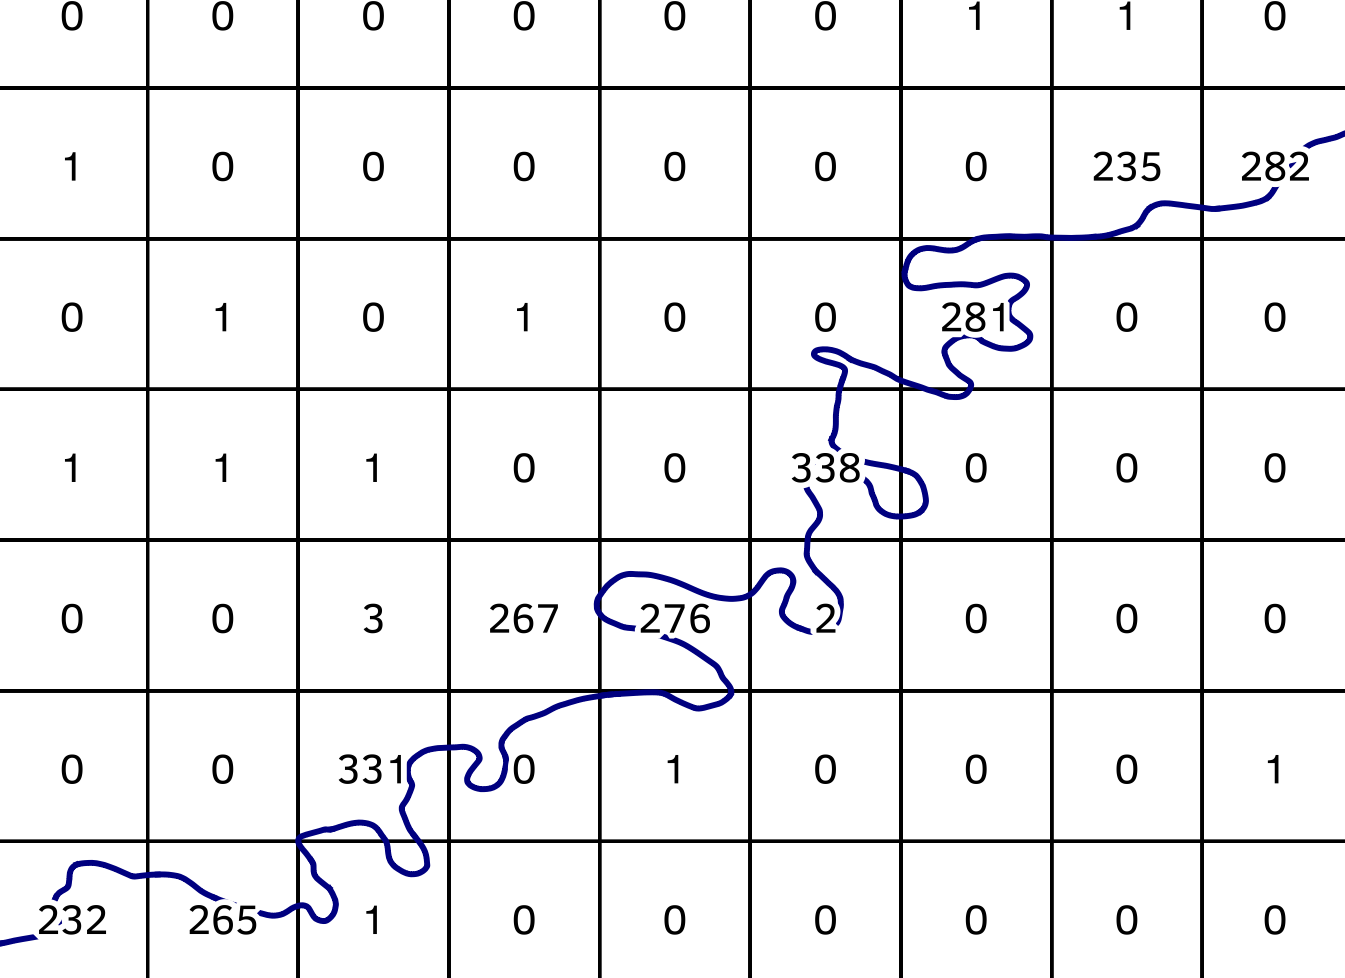
\includegraphics[width=7cm]{imp_mosel_1.png}}} \\
  \subfigure[Local maximums in the WaterGAP values]{\framebox{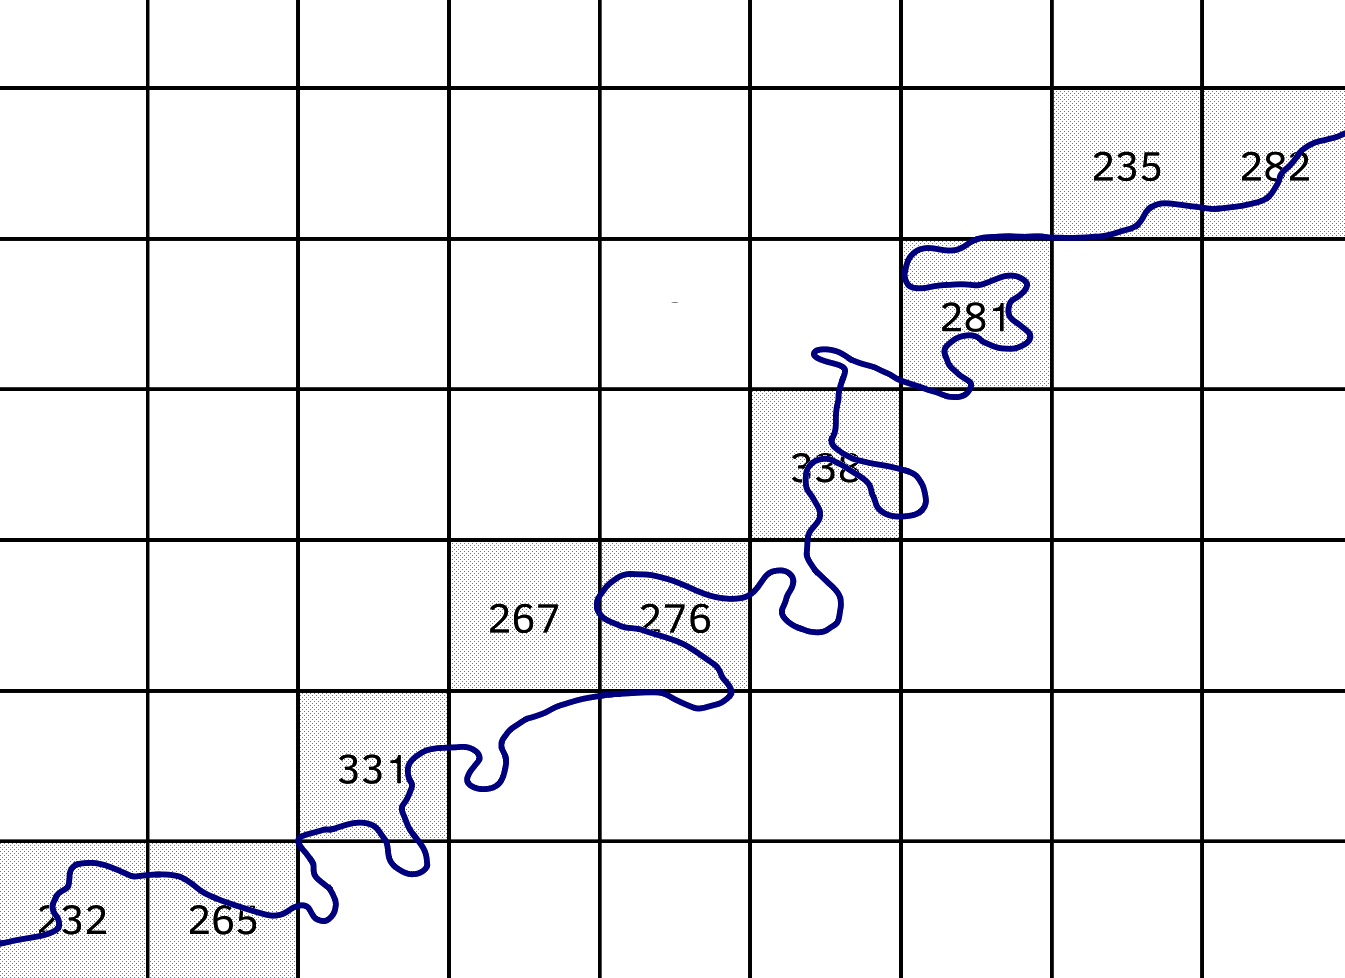
\includegraphics[width=7cm]{imp_mosel_2.png}}} \\
  \subfigure[Comparison of the course of the Mosel from WaterGAP and the DLM250]{\framebox{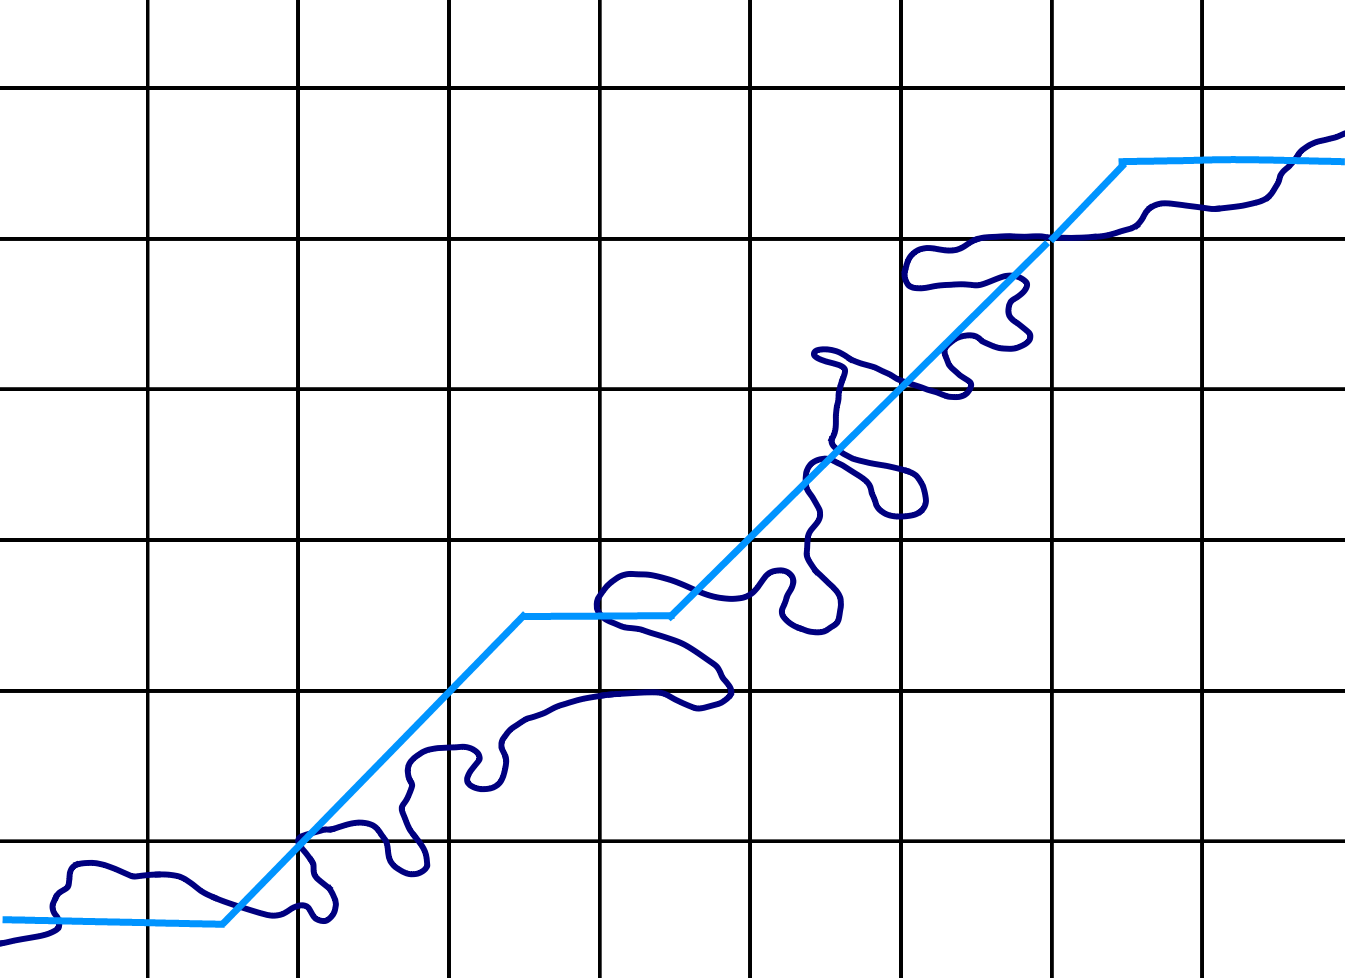
\includegraphics[width=7cm]{imp_mosel_3.png}}} 
\end{center}
\caption{River course identification for the Mosel}
\label{imp_mosel}
\end{figure}

\subsection{Residual water flow}
\label{sub:imp_dVres}
The usable runoff is obtained by subtracting the legal residual runoff from the total river runoff. Section \ref{sub:limits_others} showed that the value of the residual runoff changes a lot depending on the local law and on the year of construction of the plant, as the law changes. Therefore, to obtain a better precision, the get{\_}dV{\_}res() method (Sec. \ref{sub:getdVres}) could be amended with different ways of calculating the residual water flow, and the Modelchain class with a year and a state parameter. \newline
This requires an extended investigation into the laws of each federal state of Germany or other relevant places, but is technically easy to implement in the model and can significantly improve the precision.

\subsection{Nominal water flow and turbine type}
\label{sub:imp_dVn}
Section \ref{sub:limits_others} showed that the exceedence percentage used to calculate the nominal water flow has a big impact on the production. Since his exceedance percentage is chosen by the operator of the plant during the design process and depends on human decisions, it is difficult to chose it precisely. It would be interesting to see if a correlation can be found between the nominal power and the nominal water flow: if \unit[20]{\%} seems to be an acceptable value for big plants like the ones on the Mosel, the smaller HydroRaon seems to have been designed to work at full load \unit[30]{\%} of the time. To do so, the design parameters of a large quantity of plants have to be gathered and analyzed. This is very time-consuming, but will bring a lot to the precision of the model and to the understanding of hydro power in Germany. \newline
It would also allow a better assignment of turbine types for plants whose nominal head and nominal water flow place in the characteristic diagrams of two turbine types, as suggested in Sec. \ref{sub:limits_others}. For plants in these areas, one of the two possible types could be assigned, with a bigger probability for turbines effectively more present in this range of heads and water flows.

\subsection{Marktstammdatenregister}
\label{sub:imp_data}
The Marktstammdatenregister (MaStR) is managed by the German Federal Network Agency (BNetzA) and will constitute a complete and official register of the electricity and gas markets. It will provide a consistent and quality data set of power plants to all actors of the energy sector. It is likely that the publication of the MaStR will avoid the problems encountered in Sec. \ref{sec:db_hydroelec}. It would be very useful to have access to more precise production data as well, separated by technologies and with a good temporal definition.

\subsection{Impoudment of water}
\label{sub:impoudment}
Even though the production of run-of-the-river hydropower plants is mostly proportional to the river flow and the water impoundment created by the dam is small, it can be used to regulate the water flow in the turbine during seasons with low water flows: in order to have the turbine and the generator working at an optimal efficiency, the user should favor an operation alternating between a loading phase where water is impounded upstream from the turbine and a production phase where the water is released into the turbine with an optimal water flow and head, rather than having the system run constantly at a very low load, with little to no production due to the inefficiency of the turbine and generator at small loads. \newline
This can be implemented into the model by fixing a threshold for the river usable water flow, under which this water flow is impounded rather than flowing through the turbine. The available water flow at each timestep would then be assessed from the usable river water flow and the impounded water. This would improve the precision of the model for months with low runoffs, such as the month of August in the example of the HydroRaon turbine presented in Sec. \ref{sec:res_single}, and avoid underestimating the production of these months.
